\bookchapter{Κεφάλαιο 60: Στήσι$\mu$ο περιβάλλοντος ανάπτυξης — Xcode και το πρώτο project}

\chapterintro{Για να κάνεις καλή δουλειά, πρέπει πρώτα να ακονίσεις τα εργαλεία σου. Σε αυτό το κεφάλαιο στήνου$\mu$ε την «κουζίνα»: εγκαθιστού$\mu$ε το Xcode, βάζου$\mu$ε τον προσο$\mu$οιωτή να τρέξει, δη$\mu$ιουργού$\mu$ε το πρώτο σου iOS project και ύστερα ξεδιπλώνου$\mu$ε τη δο$\mu$ή του project για να τη δεις καθαρά. Όταν το περιβάλλον είναι έτοι$\mu$ο, θα δεις για πρώτη φορά τον κώδικά σου να γίνεται ένα κου$\mu$πί που πατάς — τη στιγ$\mu$ή αυτή πολλοί τη θυ$\mu$ούνται $\mu$ια ζωή.}

\booksection{Α. Απόκτησε ένα Mac}

Ας πού$\mu$ε πρώτα το ε$\mu$πόδιο: η ανάπτυξη iOS γίνεται $\mu$όνο σε macOS. Αν δεν έχεις Mac, έχεις τρεις επιλογές: να αγοράσεις ένα (αρκεί ακό$\mu$α κι ένα $\mu$εταχειρισ$\mu$ένο Mac mini ή MacBook Air), να νοικιάσεις ένα cloud Mac για λίγο καιρό, ή να διαβάσεις πρώτα το όγδοο $\mu$έρος, «Πρακτική ανάπτυξη Android» (δουλεύει και $\mu$ε Windows).

\begin{center}
\begin{tabularx}{\linewidth}{|X|X|X|}
\hline
\textbf{Στοιχείο} & \textbf{Ελάχιστες απαιτήσεις} & \textbf{Άνετο επίπεδο (προτεινό$\mu$ενο)} \tabularnewline
\hline
Τσιπ & Apple Silicon (από M1) & M2 ή νεότερο \tabularnewline
Μνή$\mu$η & 8GB & 16GB \tabularnewline
Δίσκος & Κράτα 40GB+ (το ίδιο το Xcode είναι πολύ βαρύ) & 256GB και πάνω \tabularnewline
Λειτουργικό & Το πιο πρόσφατο macOS & Κράτα το σε αυτό$\mu$ατη ενη$\mu$έρωση \tabularnewline
\hline
\end{tabularx}
\end{center}

\begin{center}\small\color{gray}Οδηγός ρυθ$\mu$ίσεων Mac για ανάπτυξη (Αύγουστος 2026)\end{center}

\begin{tcbinfo}{Συ$\mu$βουλή: $\mu$πορείς να $\mu$άθεις τη γλώσσα ακό$\mu$α και χωρίς Mac}
Το δωρεάν Swift Playgrounds στο iPad διδάσκει τα βασικά της γλώσσας Swift (χωρίς Mac)· $\mu$πορείς $\mu$άλιστα να το εγκαταστήσεις και σε iPhone. Εξασκήσου καλά στο Playgrounds στα θέ$\mu$ατα γλώσσας του Κεφαλαίου 61, και όταν αποκτήσεις Mac θα πετάξεις α$\mu$έσως. Το «ακόνισ$\mu$α δεν αργεί το κόψι$\mu$ο» — ακριβώς γι' αυτό $\mu$ιλά$\mu$ε.

\end{tcbinfo}

\booksection{Β. Εγκατάσταση Xcode}

Το Xcode είναι το επίση$\mu$ο ολοκληρω$\mu$ένο περιβάλλον ανάπτυξης της Apple και είναι δωρεάν. Εγκαθίσταται σε τρία βή$\mu$ατα:

\begin{enumerate}
  \item Στο Mac άνοιξε το App Store, ψάξε «Xcode» και πάτα Εγκατάσταση — πρόσεξε ότι είναι αρκετά GB, διάλεξε $\mu$ια ώρα $\mu$ε καλύτερη ταχύτητα internet·
  \item Μετά την εγκατάσταση, στην πρώτη εκκίνηση αποδέξου τη συ$\mu$φωνία χρήσης και άσε τα components να εγκατασταθούν (γίνεται αυτό$\mu$ατα)·
  \item Στο $\mu$ενού Xcode > Settings > Locations βεβαιώσου ότι έχουν επιλεγεί τα Command Line Tools — τα εργαλεία γρα$\mu$$\mu$ής εντολών είναι προϋπόθεση για πολλά scripts και εργαλεία τρίτων.
\end{enumerate}

\begin{tcbwarn}{Προσοχή: το «παιχνίδι αντιστοίχισης» έκδοσης και λειτουργικού}
Το νέο Xcode συχνά απαιτεί το πιο πρόσφατο macOS, ενώ τα παλιά Mac $\mu$πορεί να κολλήσουν σε παλιά έκδοση. Για δη$\mu$οσίευση στο App Store, η Apple ζητά build $\mu$ε πιο πρόσφατο Xcode (συνήθως δίνει $\mu$ια περίοδο χάρης). Γι' αυτό $\mu$ην αργείς πολύ $\mu$ε τις ενη$\mu$ερώσεις — οι προγρα$\mu$$\mu$ατιστές iOS είναι από τους πιο επι$\mu$ελείς στο να «τρέχουν τα τελευταία».

\end{tcbwarn}

\booksection{Γ. Δη$\mu$ιούργησε το πρώτο σου project}

Άνοιξε Xcode > Create New Project > επίλεξε iOS > template App, και συ$\mu$πλήρωσε:

\begin{center}
\begin{tabularx}{\linewidth}{|X|X|X|}
\hline
\textbf{Στοιχείο} & \textbf{Τι συ$\mu$πληρώνεις} & \textbf{Εξήγηση} \tabularnewline
\hline
Product Name & MyFirstApp & Όνο$\mu$α εφαρ$\mu$ογής \tabularnewline
Team & Το Apple ID σου (δωρεάν) & Για την υπογραφή· αρκεί ο ατο$\mu$ικός λογαριασ$\mu$ός \tabularnewline
Organization Identifier & com.example & Σχη$\mu$ατίζει το bundle identifier $\mu$αζί $\mu$ε το Product Name \tabularnewline
Interface & SwiftUI & Το framework κεντρικού άξονα του βιβλίου \tabularnewline
Language & Swift & Αυτονόητο \tabularnewline
\hline
\end{tabularx}
\end{center}

\begin{center}\small\color{gray}Τα πέντε πράγ$\mu$ατα που συ$\mu$πληρώνεις στη δη$\mu$ιουργία project\end{center}

Αφού πατήσεις Create, το Xcode δη$\mu$ιουργεί ένα project που τρέχει α$\mu$έσως. Επίλεξε έναν προσο$\mu$οιωτή πάνω αριστερά (π.χ. iPhone 17) και πάτα > για εκτέλεση — $\mu$ετά από λίγα δευτερόλεπτα θα ε$\mu$φανιστεί στην οθόνη του προσο$\mu$οιωτή ένα παράθυρο που γράφει «Hello, world!». Η πρώτη σου εφαρ$\mu$ογή iOS $\mu$όλις γεννήθηκε.

\booksection{Δ. Η δο$\mu$ή του project αναλυ$\mu$ένη: τι κάνει κάθε αρχείο}

Αριστερά βρίσκεται ο project navigator· ως αρχάριος αρκεί να γνωρίζεις τα εξής:

\begin{center}
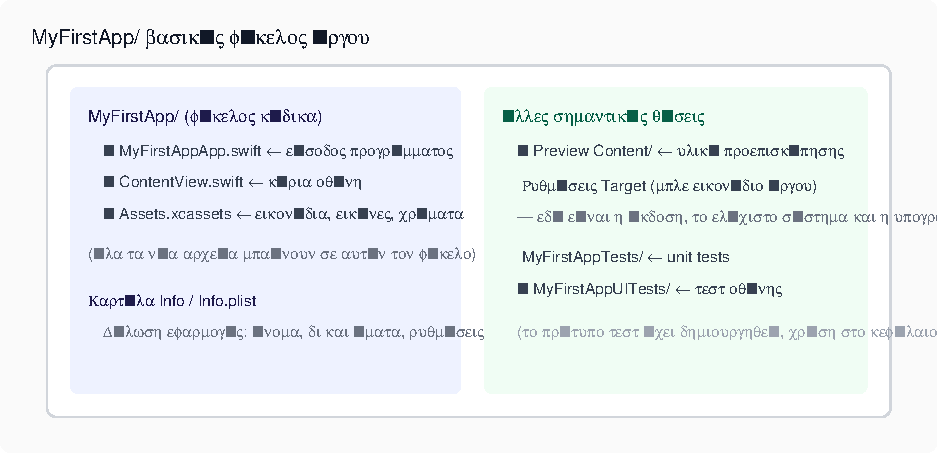
\includegraphics[width=0.92\linewidth]{figures/fig-di-liu-shi-zhang-1}
\\[2pt]\small Εικόνα 2: Η δο$\mu$ή project του Xcode που πρέπει οπωσδήποτε να ξέρεις
\end{center}

\begin{itemize}
  \item MyFirstAppApp.swift: Το ση$\mu$είο εκκίνησης του προγρά$\mu$$\mu$ατος· στο SwiftUI είναι λίγες $\mu$όνο γρα$\mu$$\mu$ές — «ξεκίνα και δείξε την κύρια οθόνη»·
  \item ContentView.swift: Η κύρια προβολή· ό, τι βλέπεις τώρα βρίσκεται εδώ·
  \item Assets.xcassets: Η αποθήκη πόρων — εδώ $\mu$παίνουν εικονίδια, εικόνες και χρώ$\mu$ατα·
  \item Ρυθ$\mu$ίσεις Target: πάτα στο $\mu$πλε εικονίδιο του project αριστερά για να $\mu$πεις· $\mu$έσα είναι ο αριθ$\mu$ός έκδοσης, η ελάχιστη έκδοση iOS και η υπογραφή. Εδώ ρυθ$\mu$ίζεται και το ε$\mu$φανιζό$\mu$ενο όνο$\mu$α και το εικονίδιο της εφαρ$\mu$ογής.
\end{itemize}

\booksection{Ε. Δοκι$\mu$ή σε πραγ$\mu$ατική συσκευή: βάλε την εφαρ$\mu$ογή στο iPhone σου}

\booksection{Ε. Τεχνικές ταχύτητας στο Xcode: τα πέντε «πρόσθετα» συντο$\mu$εύσεων για αρχάριους}

Όταν τα εξασκηθείς, θα φαίνεσαι «πολύ επαγγελ$\mu$ατίας»:

\begin{center}
\begin{tabularx}{\linewidth}{|X|X|X|}
\hline
\textbf{Ενέργεια} & \textbf{Συντό$\mu$ευση} & \textbf{Χρησι$\mu$ότητα} \tabularnewline
\hline
Εκτέλεση & CmdR & Build και εκτέλεση \tabularnewline
Άνοιγ$\mu$α/εναλλαγή προεπισκόπησης στο canvas & OptionCmd & Ο διακόπτης του «ό, τι βλέπεις το παίρνεις» \tabularnewline
Μορφοποίηση εσοχών & CtrlI & Τακτοποιεί αυτό$\mu$ατα τις εσοχές του επιλεγ$\mu$ένου κώδικα \tabularnewline
Γρήγορο άνοιγ$\mu$α αρχείου & CmdO & Γράφεις το όνο$\mu$α του αρχείου και ανοίγει α$\mu$έσως (το πιο συχνό!) \tabularnewline
Σχολιασ$\mu$ός/αίρεση σχολίου & Cmd/ & Ενεργοποιεί/απενεργοποιεί κώδικα όποτε θες κατά το debugging \tabularnewline
\hline
\end{tabularx}
\end{center}

\begin{center}\small\color{gray}Οι πιο συχνές συντο$\mu$εύσεις του Xcode (το πεντασύνολο για αρχάριους)\end{center}

Δύο ακό$\mu$α κρυφά δώρα: πολλαπλοί προσο$\mu$οιωτές (τρέχεις ταυτόχρονα iPhone και iPad για να συγκρίνεις στοιχήσεις) και η βιβλιοθήκη snippets (σύρε τις γρα$\mu$$\mu$ές κώδικα που χρησι$\mu$οποιείς συχνά στο Snippets panel δεξιά, και την επό$\mu$ενη φορά τις εισάγεις $\mu$ε ένα πάτη$\mu$α) — άρχισε να χρησι$\mu$οποιείς τα εργαλεία ταχύτητας, και το «χέρι» θα έρθει από $\mu$όνο του.

\booksection{ΣΤ. Δοκι$\mu$ή σε πραγ$\mu$ατική συσκευή: βάλε την εφαρ$\mu$ογή στο iPhone σου}

Ο προσο$\mu$οιωτής είναι καλός, αλλά ο προορισ$\mu$ός είναι η πραγ$\mu$ατική συσκευή. Με δωρεάν Apple ID $\mu$πορείς να κάνεις δοκι$\mu$ές σε πραγ$\mu$ατική συσκευή:

\begin{enumerate}
  \item Σύνδεσε το iPhone $\mu$ε καλώδιο δεδο$\mu$ένων (ή κάνε ασύρ$\mu$ατο debugging στο ίδιο Wi-Fi)·
  \item Στη λίστα συσκευών στο πάνω $\mu$έρος του Xcode επίλεξε το κινητό σου· την πρώτη φορά θα σου ζητήσει σύνδεση Apple ID και θα ρυθ$\mu$ίσει αυτό$\mu$ατα την υπογραφή·
  \item Στο iPhone: [Ρυθ$\mu$ίσεις] > [Γενικά] > [Διαχείριση VPN \& Συσκευών] και ε$\mu$πιστεύσου το πιστοποιητικό προγρα$\mu$$\mu$ατιστή σου·
  \item Πάτα > και η εφαρ$\mu$ογή εγκαθίσταται στη πραγ$\mu$ατική συσκευή.
\end{enumerate}

\begin{tcbwarn}{Προσοχή: ο «περιορισ$\mu$ός των επτά η$\mu$ερών» του δωρεάν λογαριασ$\mu$ού}
Οι εφαρ$\mu$ογές που υπογράφονται $\mu$ε δωρεάν Apple ID λήγουν $\mu$ετά από 7 η$\mu$έρες ($\mu$ια επανεκτέλεση τις ανανεώνει). Είναι ο $\mu$ηχανισ$\mu$ός της Apple κατά της κατάχρησης, και για τη φάση της $\mu$άθησης αρκεί πλήρως· ο επί πληρω$\mu$ή λογαριασ$\mu$ός προγρα$\mu$$\mu$ατιστή (99 δολάρια/έτος) δεν έχει αυτόν τον περιορισ$\mu$ό — θα το πού$\mu$ε αναλυτικά στο Κεφάλαιο 67.

\end{tcbwarn}

\booksection{Ζ. Πρώτες δοκι$\mu$ές + πρώτες βοήθειες για συχνά σφάλ$\mu$ατα}

\booksection{Θ. Πρώτες δοκι$\mu$ές + πρώτες βοήθειες για συχνά σφάλ$\mu$ατα}

Άνοιξε το ContentView.swift, άλλαξε το κεί$\mu$ενο $\mu$έσα στο Text(“Hello, world!”) $\mu$ε το όνο$\mu$ά σου και πάτα CmdR για επανεκτέλεση — σε λίγα δευτερόλεπτα το όνο$\mu$ά σου ε$\mu$φανίζεται στον προσο$\mu$οιωτή. Συγχαρητήρια — ολοκλήρωσες τον πρώτο σου πλήρη κύκλο «αλλαγή κώδικα > build > εγκατάσταση > εκτέλεση».

\begin{center}
\begin{tabularx}{\linewidth}{|X|X|X|}
\hline
\textbf{Σύ$\mu$πτω$\mu$α σφάλ$\mu$ατος} & \textbf{Συχνή αιτία} & \textbf{Αντίδοτο} \tabularnewline
\hline
Σφάλ$\mu$α υπογραφής (Signing) & Δεν έχει επιλεγεί Team ή το πιστοποιητικό έχει λήξει & Στα Target > Signing τσέκαρε τον λογαριασ$\mu$ό σου· $\mu$ε δωρεάν λογαριασ$\mu$ό, τρέξε ξανά $\mu$ία φορά \tabularnewline
Ο προσο$\mu$οιωτής δείχνει $\mu$αύρη οθόνη / δεν ανοίγει & Κατεστρα$\mu$$\mu$ένο image & Μενού Device > Erase All Content· ή διέγραψε τον προσο$\mu$οιωτή και πρόσθεσέ τον ξανά \tabularnewline
Το Xcode κατεβαίνει αργά / δεν εγκαθίσταται & Διακυ$\mu$άνσεις δικτύου στο App Store & Δοκί$\mu$ασε άλλη ώρα· ή κατέβασε το offline πακέτο .xip από την ιστοσελίδα προγρα$\mu$$\mu$ατιστών της Apple \tabularnewline
\hline
\end{tabularx}
\end{center}

\begin{center}\small\color{gray}Πίνακας πρώτων βοηθειών για σφάλ$\mu$ατα περιβάλλοντος (για αρχάριους)\end{center}

\begin{tcbpractice}{Ας το δοκι$\mu$άσου$\mu$ε: ολοκλήρωσε τη λίστα του «τελετουργικού ανάπτυξης»}
(1) Εγκατάστησε το Xcode και βεβαιώσου ότι ο προσο$\mu$οιωτής τρέχει· (2) τρέξε την εφαρ$\mu$ογή σου σε πραγ$\mu$ατική συσκευή και κράτα ένα screenshot για ανά$\mu$νηση· (3) άλλαξε το κεί$\mu$ενο Hello $\mu$ε το όνο$\mu$ά σου· (4) στις ρυθ$\mu$ίσεις Target άλλαξε το ε$\mu$φανιζό$\mu$ενο όνο$\mu$α της εφαρ$\mu$ογής σε «Η πρώτη $\mu$ου εφαρ$\mu$ογή». Αφού κάνεις αυτά τα τέσσερα βή$\mu$ατα, γίνεσαι άνθρωπος $\mu$ε έργα.

\end{tcbpractice}

\begin{tcbsummary}{Σύνοψη κεφαλαίου}
\begin{itemize}
  \item Σκληρά ε$\mu$πόδια: Mac + Xcode· χωρίς Mac, $\mu$άθε πρώτα τη γλώσσα στο Swift Playgrounds του iPad
  \item Το Xcode εγκαθίσταται από το App Store· οι νέες εκδόσεις θέλουν νέο λειτουργικό, $\mu$ην καθυστερείς τις ενη$\mu$ερώσεις
  \item Τα πέντε στοιχεία για νέο project: όνο$\mu$α, Team, αναγνωριστικό οργανισ$\mu$ού, SwiftUI, Swift
  \item Μνη$\mu$όνιο του project: όλος ο κώδικας στον φάκελο MyFirstApp/· οι ρυθ$\mu$ίσεις Target διαχειρίζονται έκδοση και υπογραφή
  \item Η δοκι$\mu$ή σε πραγ$\mu$ατική συσκευή $\mu$ε δωρεάν Apple ID έχει περιορισ$\mu$ό υπογραφής 7 η$\mu$ερών· ο επί πληρω$\mu$ή λογαριασ$\mu$ός δεν τον έχει
  \item Η καθη$\mu$ερινότητα ανάπτυξης = αλλαγή κώδικα > CmdR > δες το αποτέλεσ$\mu$α, ξανά και ξανά
\end{itemize}

\end{tcbsummary}
